\documentclass[letterpaper,11pt]{article}
\oddsidemargin -1.0cm \textwidth 17.5cm

\usepackage[utf8]{inputenc}
\usepackage[activeacute,spanish, es-lcroman]{babel}
\decimalpoint
\usepackage{amsfonts,setspace}
\usepackage{amsmath}
\usepackage{amssymb, amsmath, amsthm}
\usepackage{comment}
\usepackage{float}
\usepackage{amssymb}
\usepackage{dsfont}
\usepackage{anysize}
\usepackage{multicol}
\usepackage{enumerate}
\usepackage{graphicx}
\usepackage[left=1.5cm,top=2cm,right=1.5cm, bottom=1.7cm]{geometry}
\setlength\headheight{1.5em} 
\usepackage{fancyhdr}
\usepackage{multicol}
\usepackage{hyperref}
\usepackage{wrapfig}
\usepackage{subcaption}
\usepackage{siunitx}
\usepackage{cancel}
\usepackage{mdwlist}
\usepackage{svg}
\pagestyle{fancy}
\fancyhf{}
\renewcommand{\labelenumi}{\normalsize\bfseries P\arabic{enumi}.}
\renewcommand{\labelenumii}{\normalsize\bfseries (\alph{enumii})}
\renewcommand{\labelenumiii}{\normalsize\bfseries \roman{enumiii})}


\begin{document}

\fancyhead[L]{\itshape{Facultad de Ciencias F\'isicas y Matem\'aticas}}
\fancyhead[R]{\itshape{Universidad de Chile}}
\rfoot[]{pág. \thepage}

\begin{minipage}{11.5cm}
    \begin{flushleft}
        \hspace*{-0.6cm}\textbf{FI1000-1 Introducción a la Física Clásica}\\
        \hspace*{-0.6cm}\textbf{Profesor:} Ignacio Bordeu\\
        \hspace*{-0.6cm}\textbf{Auxiliares:} Alejandro Cartes \& Simón Yáñez\\
        \hspace*{-0.6cm}\textbf{Ayudante:} Javier Cubillos\\
    \end{flushleft}
\end{minipage}

\begin{picture}(2,3)
    \put(366, 10){
\includegraphics[scale=0.9]{2020-1/Imágenes/logo/dfi-fcfm.pdf}}
\end{picture}

\begin{center}
	\LARGE\textbf{Auxiliar \#10+1}\\
	\Large{+ momentum}
\end{center}

\vspace{-1cm}
\begin{enumerate}\setlength{\itemsep}{0.4cm}

\item[]

% se guarda
% \item \textbf{[P2-C3 2017-1]} Un bloque de masa $M$ con una superficie superior con la forma de medio cilindro de radio $R$ se encuentra sobre una superficie horizontal sin rozamiento al tiempo que toca un muro vertical en su lado izquierdo. Una partícula de masa $m$ se suelta desde el extremo superior izquierdo de la cavidad como se muestra en la figura. Suponiendo que la fricción puede despreciarse:
% \begin{enumerate}
%     \item Determine la rapidez de la partícula al llegar por primera vez a la parte más baja de su trayectoria
    
%     \item Examine cualitativamente la acción de la fuerza normal del muro sobre el bloque de masa $M$ y determine el instante a partir del cual el bloque se desliza a la derecha. Para tiempos posteriores a este, ¿qué principio de conservación utiliza?
    
%     \item Determine la rapidez máxima que alcanza el bloque en su movimiento desoués de soltar la masita $m$
% \end{enumerate}

% \begin{figure}[H]
%     \centering
%     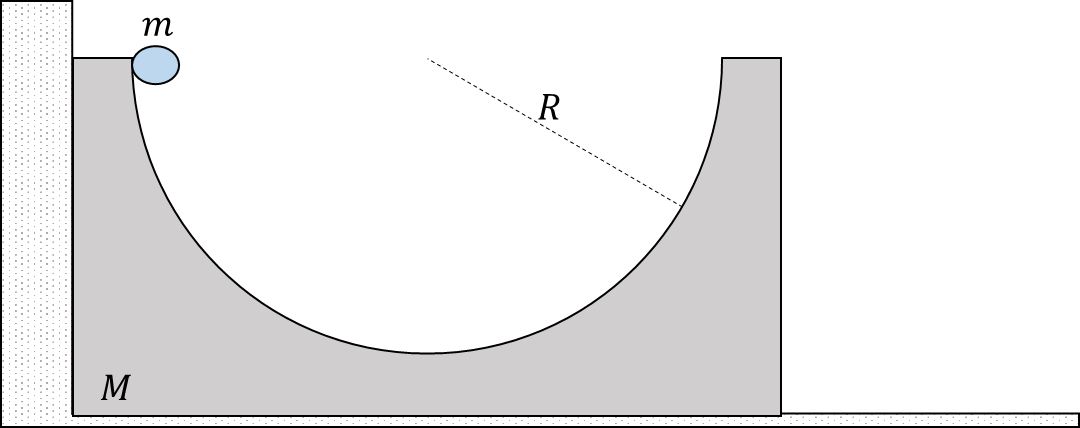
\includegraphics[width=0.5\linewidth]{2023-1/img/aux_11/bloque-p.png}
% \end{figure}

\item Un objeto de masa $m$ resbala sobre la superficie lisa de una cuña de masa $M$. La cuña reposa sobre una superficie lisa. Inicialmente el objeto se encuentra en reposo a una altura $h$ medida desde el tramo horizontal.

\begin{multicols}{2}
    
    \begin{enumerate}
        \item Calcule las velocidades de la cuña y de la masa $m$ una vez que $m$ ha llegado al tramo horizontal de la cuña y esté desplazándose hacia la derecha.
        
        \item Posteriormente, la masa $m$ choca elásticamente con la parte posterior de la cuña. Calcule la rapidez de $m$ y $M$ después del choque.
    \end{enumerate}
    
    \columnbreak
    
    \begin{figure}[H]
        \centering
        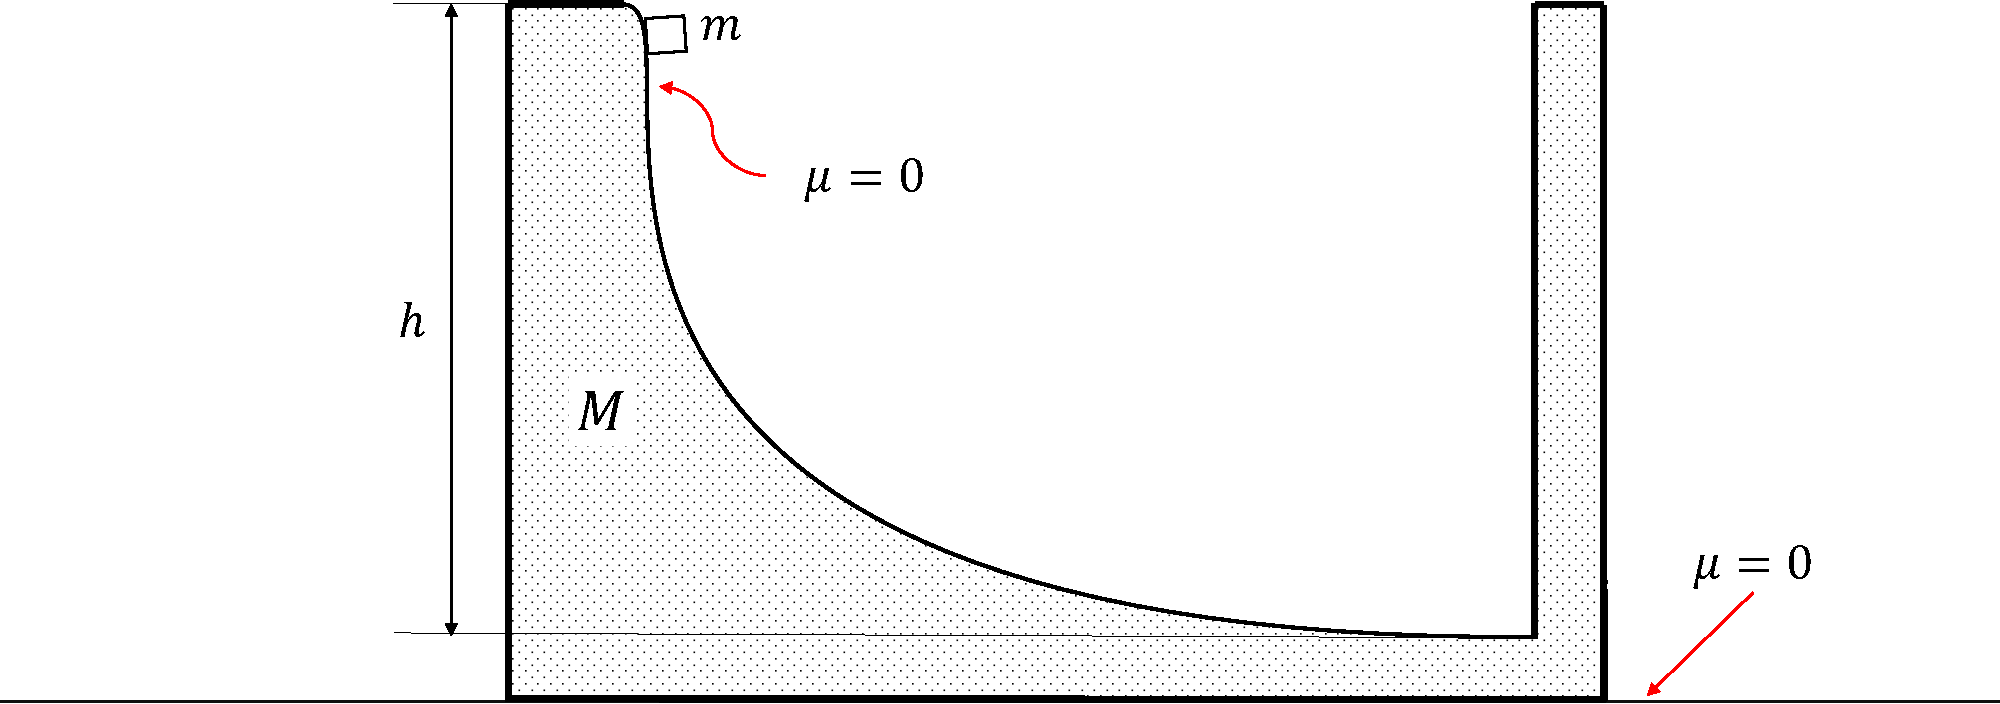
\includegraphics[width=1\linewidth]{2020-1/Imágenes/aux13/cuna.pdf}
    \end{figure}

\end{multicols}
\begin{multicols}{2}
    \item Un balín de masa $m$ y rapidez inicial $v_0$ pasa a través de un bloque de masa $M$ que está colgado por una cuerda ideal de largo $L$ como se muestra en la figura. El balín, tras la colisión, sale con rapidez $v_1$. El suceso ocurre muy rápido y la masa del bloque permanece constante (i.e. la masa perdida del agujero es despreciable). Determine el ángulo $\theta_{max}$ alcanzado por el bloque.
    
    \columnbreak
    
    \begin{figure}[H]
        \centering
        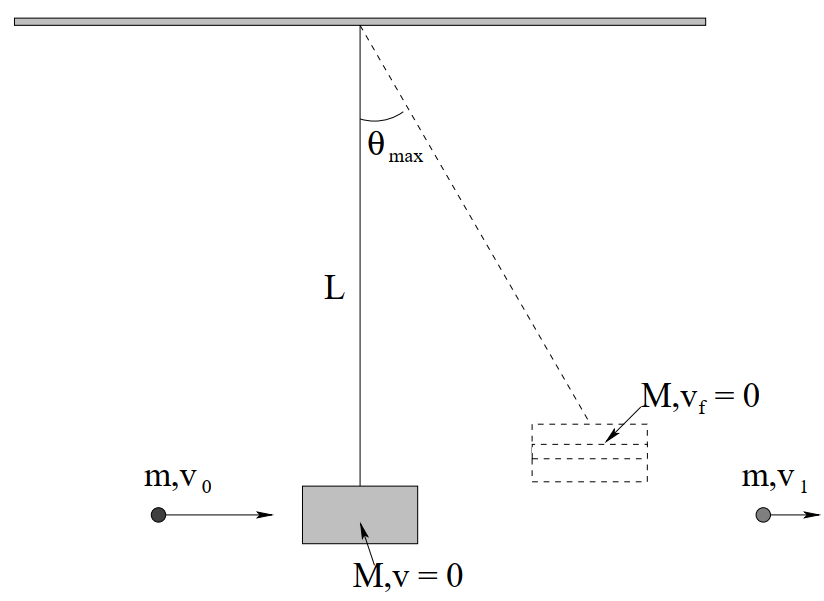
\includegraphics[width=0.7\linewidth]{2023-1/img/aux_11/pendulo-balistico.png}
    \end{figure}
\end{multicols}

\begin{multicols}{2}
    \item Considere un bloque de masa $m$ sostenido por dos resortes de largo natural nulo y con constantes elásticas $k_1$ y $k_2$ como se muestra en la figura. Una vez que el sistema alcanza el equilibrio, se lanza un proyectil de masa $m$ a una velocidad $v$. Si el proyectil y el bloque terminan viajando juntos, determine:

    \begin{enumerate}
        \item La elongación de cada resorte en el equilibrio (pre-colisión).
        
        \item La máxima elongación de cada resorte tras la colisión. Considere que el sistema proyectil-bloque se mueve horizontalmente.
    \end{enumerate}
    
    \columnbreak
    
    \begin{figure}[H]
        \centering
        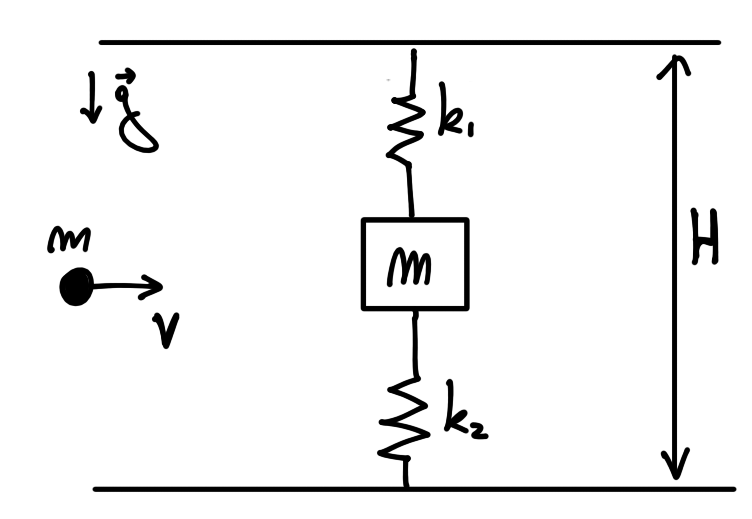
\includegraphics[width=0.9\linewidth]{2023-1/img/aux_11/p3c2.png}
    \end{figure}
\end{multicols}
\textbf{\textit{Hint}}: Encuentre la relación geométrica entre las elongaciones de los resortes pre-colisión y una vez que el sistema ha alcanzado la máxima elongación. Note los triángulos rectángulos que se forman.  

% Para imágenes vectoriales -> el texto tiene que estar en LaTeX
% \begin{figure}[htbp]
%   \centering
%   \svgpath{../Imagenes/ejercicios}  -> .. irse pa'trás 
%   \includesvg{ej5.svg}
% \end{figure}

\end{enumerate}
\end{document}
